\documentclass{beamer}

\usepackage{graphics}
\usepackage{graphicx}
\usepackage{float}
\usepackage{caption}
\usepackage{subcaption}
\usepackage{color}

% black theme: 
\setbeamercolor{background canvas}{bg=black}
\setbeamercolor{normal text}{fg=white}
\setbeamercolor{title}{fg=white}
\setbeamercolor{frametitle}{fg=white}
\setbeamercolor{structure}{fg=white}

% burgundy and white theme:
%\usetheme{Szeged}
%\usecolortheme{beaver}

\beamertemplatenavigationsymbolsempty
\frenchspacing
\setbeamertemplate{itemize item}{\color{black}\textbullet}
\usefonttheme{serif}

\captionsetup[figure]{labelformat=empty}
\captionsetup[subfigure]{labelformat=empty}

\newcommand\frametitlesc[1]{\frametitle{\sc #1}}

\newcommand\prn[1]{\left( #1 \right)}
\newcommand\set[1]{\left\{ #1 \right\}}
\newcommand\ee{\boldsymbol{e}}
\newcommand\yy{\boldsymbol{y}}
\newcommand\YY{\boldsymbol{Y}}
\newcommand\RR{\mathbb{R}}
\newcommand\rf{{\mathrm{rf}}}
\newcommand\te{{\mathrm{te}}}


\title[Changepoint detection]{\sc Algorithms for detecting changepoints in data}
\author{Cody Buntain, Christopher Natoli, Miroslav \v{Z}ivkovi\'{c}}
\date{24 July 2014}
\institute[OSDC PIRE 2014 at UvA]{OSDC PIRE 2014, hosted at University of Amsterdam}

\begin{document}

\frame{\titlepage}

\section{Algorithms}

\subsection{Cusum}

\frame{
  \frametitlesc{Building the test statistic}
  $$
  \mathrm{test\;statistic}=
  \onslide<5->{\frac{h}{\sqrt{2kn}}\bigg(}
  \frac{
    \onslide<1->{\sum_{t=1}^h\ee_t}
    \onslide<2->{^\top}
    \onslide<3->{(\hat\Sigma)^{-1}}
    \onslide<2->{\ee_t}
  }{\onslide<3->{h}}
  \onslide<4->{-\frac{\sum_{t=1}^n\ee_t^\top(\hat\Sigma)^{-1}\ee_t}{n}}
  \onslide<5->{\bigg)}
  $$
  \onslide<3>{$$\hat\Sigma:=\frac{1}{n-1}\sum_{t=1}^n\ee_t\ee_t^\top$$}
  \vfill
  \tiny{Galeano, Pedro, and Daniel Pe\~{n}a. ``Covariance changes detection in multivariate time series.'' \textit{Journal of Statistical Planning and Inference} 137.1 (2007): 194-211.}
}

\frame{
  \frametitlesc{Finding a single changepoint}
  \begin{figure}
    \centering
    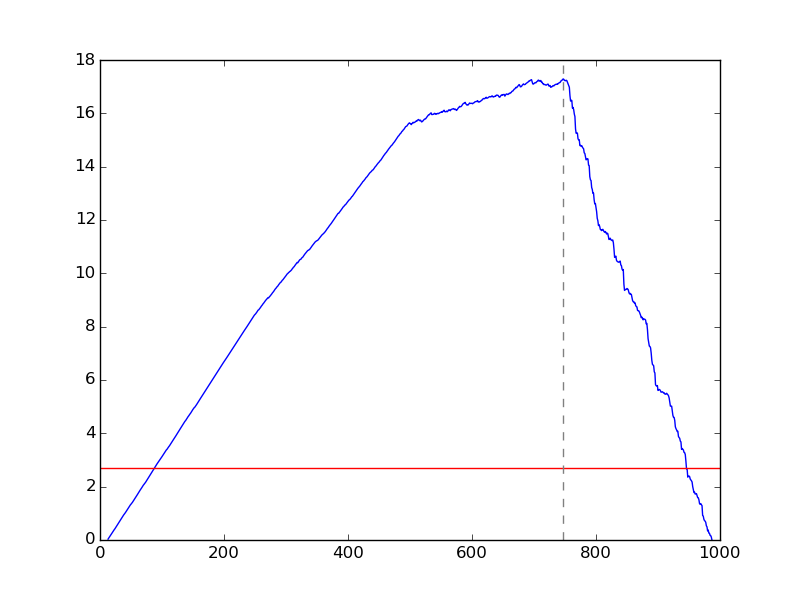
\includegraphics[width=.6\textwidth]{cusum_plot1.png}
    \caption{Cusum statistic for a time series with three changepoints.}
  \end{figure}
  \vfill
  \tiny{Galeano, Pedro, and Daniel Pe\~{n}a. ``Covariance changes detection in multivariate time series.'' \textit{Journal of Statistical Planning and Inference} 137.1 (2007): 194-211.}}

\frame{
  \frametitlesc{Finding a single changepoint}
  \footnotesize
  \begin{align*}
  \mathrm{test\;statistic}
  &=\frac{h}{\sqrt{2kn}}\bigg(\frac{\sum_{t=1}^h\ee_t^\top(\hat\Sigma)^{-1}\ee_t}{h}-\frac{\sum_{t=1}^n\ee_t^\top(\hat\Sigma)^{-1}\ee_t}{n}\bigg)\\
  \max(\mathrm{test\;statistic})
  &\xrightarrow{D}\sup\set{\text{Brownian bridge}},
  \end{align*}
  which is a known distribution, so we can compute critical values.
  \vfill
  \tiny{Galeano, Pedro, and Daniel Pe\~{n}a. ``Covariance changes detection in multivariate time series.'' \textit{Journal of Statistical Planning and Inference} 137.1 (2007): 194-211.}
}

\frame{
  \frametitlesc{Finding more changepoints}
  \begin{figure}
    \centering
    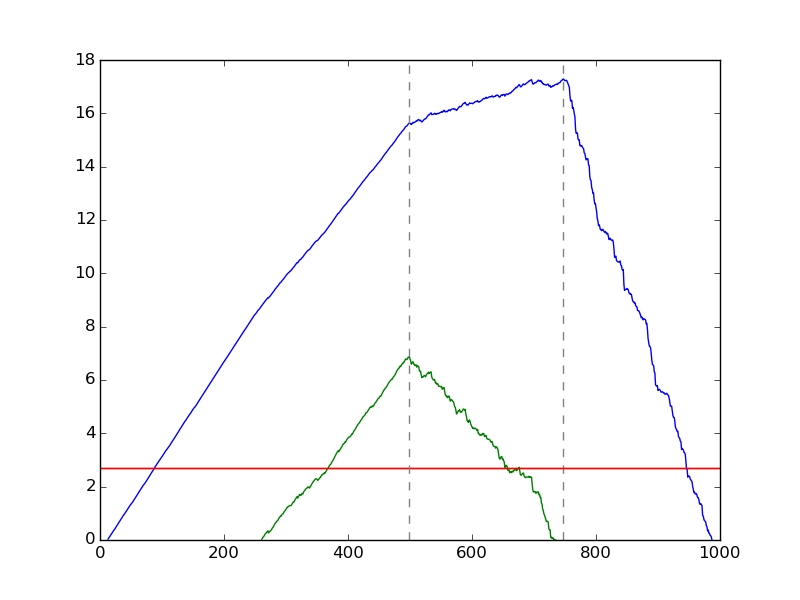
\includegraphics[width=.6\textwidth]{cusum_plot2.png}
    \caption{Cusum statistic for a time series with three changepoints.}
  \end{figure}
  \vfill
  \tiny{Galeano, Pedro, and Daniel Pe\~{n}a. ``Covariance changes detection in multivariate time series.'' \textit{Journal of Statistical Planning and Inference} 137.1 (2007): 194-211.}
}

\subsection{Density ratio estimation}

\frame{
  \frametitlesc{Moving from datapoints to subsequences}
  Suppose time series $\yy(t)\in\RR^3$ and denote its $i$th component by $y_i(t)\in\RR$.
  Define the subsequence
  $$\YY(t)=
  \begin{pmatrix}
    y_1(t)\\
    y_2(t)\\
    y_3(t)\\
    y_1(t+1)\\
    y_2(t+1)\\
    y_3(t+1)\\
    \vdots\\
    y_1(t+m-1)\\
    y_2(t+m-1)\\
    y_3(t+m-1)\\
  \end{pmatrix}.
  $$
  \vfill
  \tiny{Kawahara, Yoshinobu and Masashi Sugiyama. ``Sequential change‐point detection based on direct density‐ratio estimation.'' \textit{Statistical Analysis and Data Mining} 5.2 (2012): 114-127.}
}

\frame{
  \frametitlesc{Moving from datapoints to subsequences}
  \begin{figure}[h]
    \centering
    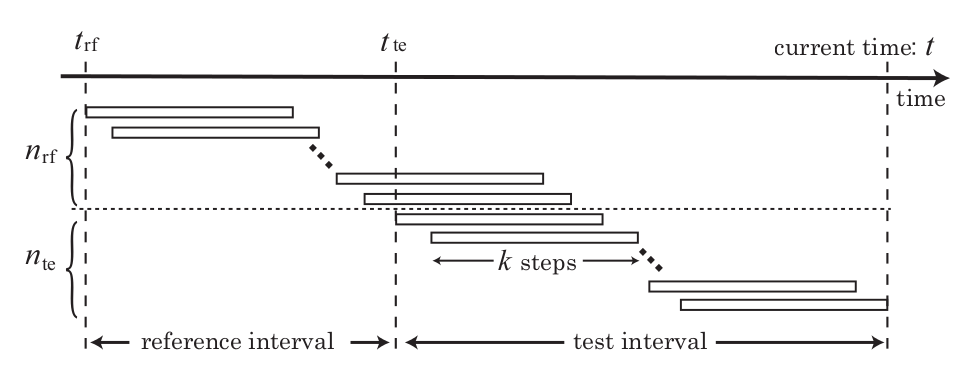
\includegraphics[width=\textwidth]{subsequence_diagram.png}
    \caption{Sliding window of subsequences.\\(Reference interval has pdf $p_\rf$ and test interval has pdf $p_\te$.)}
  \end{figure}
  \vfill
  \tiny{Kawahara, Yoshinobu and Masashi Sugiyama. ``Sequential change‐point detection based on direct density‐ratio estimation.'' \textit{Statistical Analysis and Data Mining} 5.2 (2012): 114-127.}
}

\frame{
  \frametitlesc{Hypothesis test}
  \begin{align*}
    H_0\colon&p(\YY(i))=p_\rf(Y(i))\quad\quad\text{for $i=t_\rf,\ldots,t-1$}\\
    \text{vs}\quad
    H_1\colon&p(\YY(i))=p_\rf(Y(i))\quad\quad\text{for $i=t_\rf,\ldots,t_\te-1$}\\
    &p(\YY(i))=p_\te(Y(i))\quad\quad\text{for $i=t_\te,\ldots,t-1$}.
  \end{align*}
  \onslide<2->{
    $$
    \mathrm{likelihood\;ratio}=\prod_{i=1}^{n_\te}\frac{p_\te(\YY_\te(i))}{p_\rf(\YY_\te(i))}
    $$
  }
  \vfill
  \tiny{Kawahara, Yoshinobu and Masashi Sugiyama. ``Sequential change‐point detection based on direct density‐ratio estimation.'' \textit{Statistical Analysis and Data Mining} 5.2 (2012): 114-127.}
}

\frame{
  \frametitlesc{Directly estimating the density ratio}
  \begin{align*}
    w(\YY)&=\frac{p_\te(\YY)}{p_\rf(\YY)}\\
    \onslide<2->{\hat w(\cdot)&=\sum_{\ell=1}^b\alpha_\ell\phi_\ell(\cdot)}
    \onslide<3->{=\sum_{\ell=1}^{\onslide<4->{n_\te}}\alpha_\ell K_\sigma(\cdot,\onslide<4->{\YY_\te(\ell)})}\\
  \end{align*}
  \onslide<3->{Gaussian kernel $K_\sigma(\YY,\YY')=\exp\prn{-\frac{\|\YY-\YY'\|^2}{2\sigma^2}}$}
  \vfill
  \tiny{Kawahara, Yoshinobu and Masashi Sugiyama. ``Sequential change‐point detection based on direct density‐ratio estimation.'' \textit{Statistical Analysis and Data Mining} 5.2 (2012): 114-127.}
}

\frame{
  \frametitlesc{Directly estimating the density ratio}
  $$\hat p_\te(\cdot):=p_\rf(\cdot)\hat w(\cdot)=p_\rf(\cdot)\sum_{\ell=1}^{n_\te}\alpha_\ell K_\sigma(\cdot,\YY_\te(\ell))$$
  \onslide<2->{
    \begin{align*}
      \min_{\set{\alpha_\ell}}&\quad\text{Kullback-Leibler divergence}(p_\te\|\hat p_\te)\\
      \onslide<3->{\text{subject to}&\quad\text{some uninteresting constraints}}
    \end{align*}
  }
  \vfill
  \tiny{Kawahara, Yoshinobu and Masashi Sugiyama. ``Sequential change‐point detection based on direct density‐ratio estimation.'' \textit{Statistical Analysis and Data Mining} 5.2 (2012): 114-127.}
}


\end{document}
